\section{Diffusion models samplers}
\label{appendix:dm_samplers}

Sampling from diffusion model can take thousands of denoising steps. In this section we will see common samplers used in the literature to sample from diffusion models for faster inference. First we need to establish basic mathematical grounds with the forward and reverse diffusion process as described in the DDPM paper \cite{ddpm} in the next two sections.








\subsection*{Forward process}

In the forward process we can take step-by-step approach (adding noise at each step, current step depends on previous step only):

\[ q(x_t | x_{t-1}) := \mathcal{N} \left( \sqrt{\frac{\alpha_t}{\alpha_{t-1}}} x_{t-1}, \left( 1 - \frac{\alpha_t}{\alpha_{t-1}} I \right) \right) \]

where $\alpha \in (0, 1]$ is the scaling factor of the noise scheduler, $\alpha_t$ is the noise added at timestep $t$.

However, in the DDPM paper \cite{ddpm} they showed that we can go from $x_0$ (the original image without any noise added) to $x_T$ (pure Gaussian noise) (or to that matter any arbitrary step $t$) in one step:

\[ q(x_t | x_0) := \mathcal{N} \left( x_t; \sqrt{\bar{\alpha}_t} x_0, (1 - \bar{\alpha}_t) I \right) \]

where $\bar{\alpha}_t = \prod_{s=1}^{t} \alpha_s$.

Because it is not straightforward to implement, they used the reparameterization trick:

\begin{equation}
    x_t = \sqrt{\alpha_t} x_0 + \sqrt{1 - \alpha_t} \epsilon
    \label{eq:appendix_ddpm_reparam_trick}
\end{equation}

where $\epsilon \sim \mathcal{N} (0, I)$. 








\subsection*{Backward process}

In reverse diffusion process we go from noisy image and denoise it iteratively to get the original denoised image:

\[ p_\theta (x_{0:T}) := p(x_T) \prod_{t=1}^{T} p_\theta (x_{t-1} | x_t) \]

where $p(x_T)$ is the sampled noisy image (Gaussian noise) and we iteratively multiply by the denoising procedure where each step depends on the previous step.









\subsection{DDPM / Stochastic Sampler}

% \begin{figure}
%     \centering
%     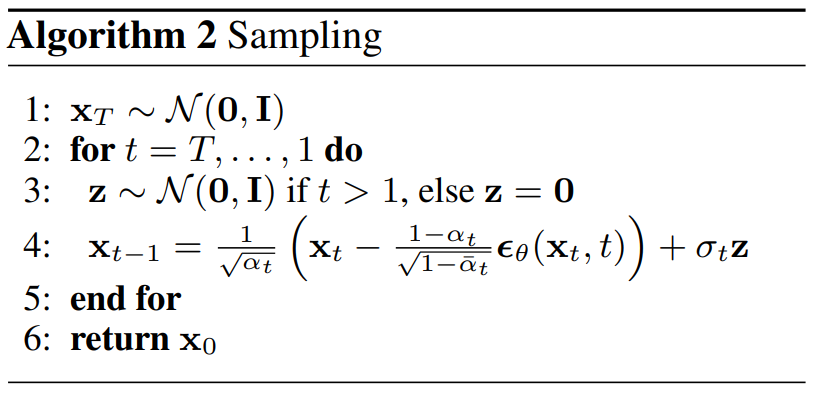
\includegraphics[width=0.3\textwidth]{images/appendix/dm_samplers/ddpm.png}
%     \caption{DDPM sampler. Sampling process from the DDPM paper \cite{ddpm}.}
%     \label{fig:appendix_ddpm_sampling}
% \end{figure}




\begin{algorithm}
    \caption{DDPM Sampling algorithm from the DDPM paper \cite{ddpm}.}
    \label{alg:appendix_ddpm_sampling}
    \begin{algorithmic}[1]
        \State $\mathbf{x}_T \sim \mathcal{N}(\mathbf{0}, \mathbf{I})$
        \For{$t = T, \dots, 1$}
            \State $\mathbf{z} \sim \mathcal{N}(\mathbf{0}, \mathbf{I})$ if $t > 1$, else $\mathbf{z} = \mathbf{0}$
            \State $\mathbf{x}_{t-1} = \frac{1}{\sqrt{\alpha_t}} \left( \mathbf{x}_t - \frac{1 - \alpha_t}{\sqrt{1 - \bar{\alpha}_t}} {\epsilon}_{\theta} (\mathbf{x}_t, t) \right) + \sigma_t \mathbf{z}$
        \EndFor
        \State \textbf{return} $\mathbf{x}_0$
    \end{algorithmic}
\end{algorithm}






The DDPM sampling algorithm is shown in algorithm \ref{alg:appendix_ddpm_sampling}: random Gaussian noise $x_T \sim \mathcal{N} (0, I)$ is first sampled, and then for $T$ iterations we slowly denoise the image:

\[ x_{t-1} = \frac{1}{\sqrt{\alpha_t}} \left( x_t - \frac{1 - \alpha_t}{\sqrt{1 - \bar{\alpha_t}}} \epsilon_\theta (x_t, t) \right) + \sigma_t z \]

where $\epsilon_\theta$ is the denoising neural network (that predicts the noise, the U-Net) with the inputs $(x_t, t)$. Then the noise is removed from the image: $\left( x_t - \frac{1 - \alpha_t}{\sqrt{1 - \bar{\alpha_t}}} \right)$. 

The last term $\sigma_t z$ is the variance to vary the samples. For instance, if $z=0$ then every time we generate an image from the same noisy image $x_T$ we get the same result (the same cat for instance). When we reach the final step $t=0$ then we set $z=0$ to get the final denoised image $x_0$ without variance.







\subsection{DDIM Sampler}

One problem of denoising an image is that there are multiple paths of the denoising steps to take; in two denoising steps, we can reach the same result but in different ways. The denoising diffusion implicit models (DDIM) paper \cite{ddim} suggest non-markovian deterministic approach to fast infer samples from the diffusion model:

\[ q_\sigma (x_{1:T} | x_0) := q_\sigma (x_T | x_0) \prod_{t=2}^{T} q_\sigma (x_{t-1} | x_t, x_0)\]

where $q_\sigma (x_T | x_0)$ is the forward process to noise an image in a single step (equation \ref{eq:appendix_ddpm_reparam_trick}). The term $q_\sigma (x_{t-1} | x_t, x_0)$ describes how to get to noisy image at timestep $t$ from the original image $x_0$ from any marginal distribution in the middle of the diffusion process given $(x_t, x_0)$ \footnote{Thanks in part to \href{https://www.youtube.com/watch?v=r4V0vLhYZIQ&t=686s}{a youtube guide} for the explanation of DDIM sampling}:

\begin{equation}
q_\sigma (x_{t-1} | x_t, x_0) = \mathcal{N} \left( 
\underbrace{
    \textcolor{red}{\sqrt{\alpha_{t-1}} x_0} + \textcolor{blue}{\sqrt{1 - \alpha_{t-1} - \sigma_t^2}} \cdot \textcolor{magenta}{\frac{x_t - \sqrt{\alpha_t} x_0}{\sqrt{1 - \alpha_t}}}
}_{
    \text{Eq. \ref{eq:appendix_ddpm_reparam_trick}:}\ x_t = \textcolor{red}{\sqrt{\alpha_t} x_0} + \textcolor{blue}{\sqrt{1 - \alpha_t}} \cdot \textcolor{magenta}{\epsilon}
}, \sigma_t^2 I 
\right)
\label{eq:appendix_ddim_q}
\end{equation}

In other words, we can achieve $x_100$ if we have $x_101, x_0$; we can achieve $x_99$ if we have $x_100, x_0$ and so on.

The underbrace term is the reparameterization trick (equation \ref{eq:appendix_ddpm_reparam_trick}). We can see that this equation is similar, the only difference is the noise term $\epsilon$: instead of stochastically sampling noise from normal distribution, it is now dependent on $x_0$ and $x_T$ and is deterministic (the term $\textcolor{magenta}{\frac{x_t - \sqrt{\alpha_t} x_0}{\sqrt{1 - \alpha_t}}}$).

Another difference between equations \ref{eq:appendix_ddim_q} and \ref{eq:appendix_ddpm_reparam_trick} is the $\sigma_t^2$ term; the role of this term is to add stochasticity. If we set $\sigma_t^2 = 0$ then we have no variance, and we deterministically traverse every intermediate noisy image $x_t$.

Using DDIM sampler the \textbf{forward process} can be derived from Bayes' rule:

\[ q_{\sigma}(\mathbf{x}_t | \mathbf{x}_{t-1}, \mathbf{x}_0) = \frac{q_{\sigma}(\mathbf{x}_{t-1} | \mathbf{x}_t, \mathbf{x}_0) q_{\sigma}(\mathbf{x}_t | \mathbf{x}_0)}{q_{\sigma}(\mathbf{x}_{t-1} | \mathbf{x}_0)} \]

The \textbf{backward process} $p_\theta^{(t)} (x_{t-1} | x_t)$ leverages the knowledge of the forward process ($q_\sigma (x_{t-1} | x_t, x_0)$):

\[ p_\theta^{(t)} (x_{t-1} | x_t) = q_\sigma (x_{t-1} | x_t, f_\theta^{(t)} (x_t)) \]

But since we don't have $x_0$ at inference time, we estimate it using our neural network $f_\theta^{(t)} (x_t)$. Our network knows only to predict noise, however we can reach $x_0$ from $x_t$ with a single step:

\[ f_\theta^{(t)} (x_t) := \left( x_t - \sqrt{1 - \alpha_t} \cdot \epsilon_\theta^{(t)} (x_t) \right) / \sqrt{\alpha_t} \]

So at each timestep $t$ our neural network has estimation of $x_0$; the larger the $t$ the more error we have (since the task of directly denoising from complete noisy image $x_T$ is more challenging than denoising from less noisy image, say $x_{10}$).

We calculate the error for $x_t$, $x_{t-1}$, and so on. The noise prediction task becomes more and more easy.

To summarize, the sampling process is described as follows:

\begin{equation}
\mathbf{x}_{t-1} = \sqrt{\alpha_{t-1}} \underbrace{\left( \frac{\mathbf{x}_t - \sqrt{1 - \alpha_t} \, \epsilon_{\theta}^{(t)}(\mathbf{x}_t)}{\sqrt{\alpha_t}} \right)}_{\text{"predicted } \mathbf{x}_0\text{"}} + \underbrace{\sqrt{1 - \alpha_{t-1} - \sigma_t^2} \cdot \epsilon_{\theta}^{(t)}(\mathbf{x}_t)}_{\text{"direction pointing to } \mathbf{x}_t\text{"}} + \underbrace{\sigma_t \, \epsilon_t}_{\text{random noise}}
\end{equation}

\begin{itemize}
    \item The first term: the neural network first predicts the noise, and then it uses the noise prediction to derive to $x_0$ from $x_t$ (possibly with a lot of error / loss).
    \item The second term: the same noise prediction $\epsilon_{\theta}^{(t)}$ is added to $x_t$ but with less severity.
    \item The third term: similar to $\sigma_t^2$ in equation \ref{eq:appendix_ddim_q}; it adds stochasticity to the sampling process.
\end{itemize}










% \subsubsection{SDE Sampler}

% ...